% Choosing the prediction horizon for traversability supervision.
% Requires: graphicx, booktabs. Figure and table are generated by
% training/traversability_network/notebooks/horizon_grid_coverage.ipynb.
\subsection{Choosing the Prediction Horizon}
\label{sec:horizon}

The network is supervised on the robot's future trajectory: for each anchor
pose the next $H$ odometry steps (at $\mathrm{d}t = 0.1\,$s) are expressed
in the anchor ego frame and projected onto the bird's-eye-view (BEV) grid, which
spans $[-2, 8]\,$m forward and $[-5, 5]\,$m laterally. Any path point that falls
outside the grid is masked by the traversability criterion.

WayFASTER uses $H = 300$ (30\,s), tuned for a wheeled robot. ANYmal moves much
more slowly, so a 30\,s path overshoots the 8\,m grid and a large fraction of it
is masked. To pick a horizon we balance two competing quantities:

\begin{description}
  \item[Coverage] The fraction of all supervised poses that fall inside the grid.
        A value of 100\,\% means nothing was masked.
  \item[Reach] The deepest forward (ego-$x$) distance the path attains
        while still inside the grid. It measures how far ahead supervision is
        actually placed.
\end{description}


The two quantities pull in opposite directions (Figure~\ref{fig:horizon},
Table~\ref{tab:horizon}). A short horizon keeps coverage near 100\,\% but the path
barely advances: at $H = 50$ the median path reaches only 2.6\,m and no anchor
reaches the far band.
Further, hazards are only labeled as such when the robot is nearly on top of them, whereas a planner must recognise them from afar.
A long
horizon improves reach but masks a growing share of the supervision (only 60\,\%
of poses are in-grid at $H = 300$) and accumulates odometry drift.
Masking is graceful, though: A short reach does not drop the patch from the dataset, it only omits the far-range views of it., so a large horizon is inefficient, not wrong.

We adopt $H = 180$ (18\,s): 79\,\% coverage, a median reach of 6.7\,m, and 55\,\%
of anchors in the desirable far band.
% The more conservative $H = 150$ (86\,\% coverage, 50\,\% past 6\,m) is a reasonable fallback if far-pose drift proves harmful.

\begin{figure}[htbp]
  \centering
  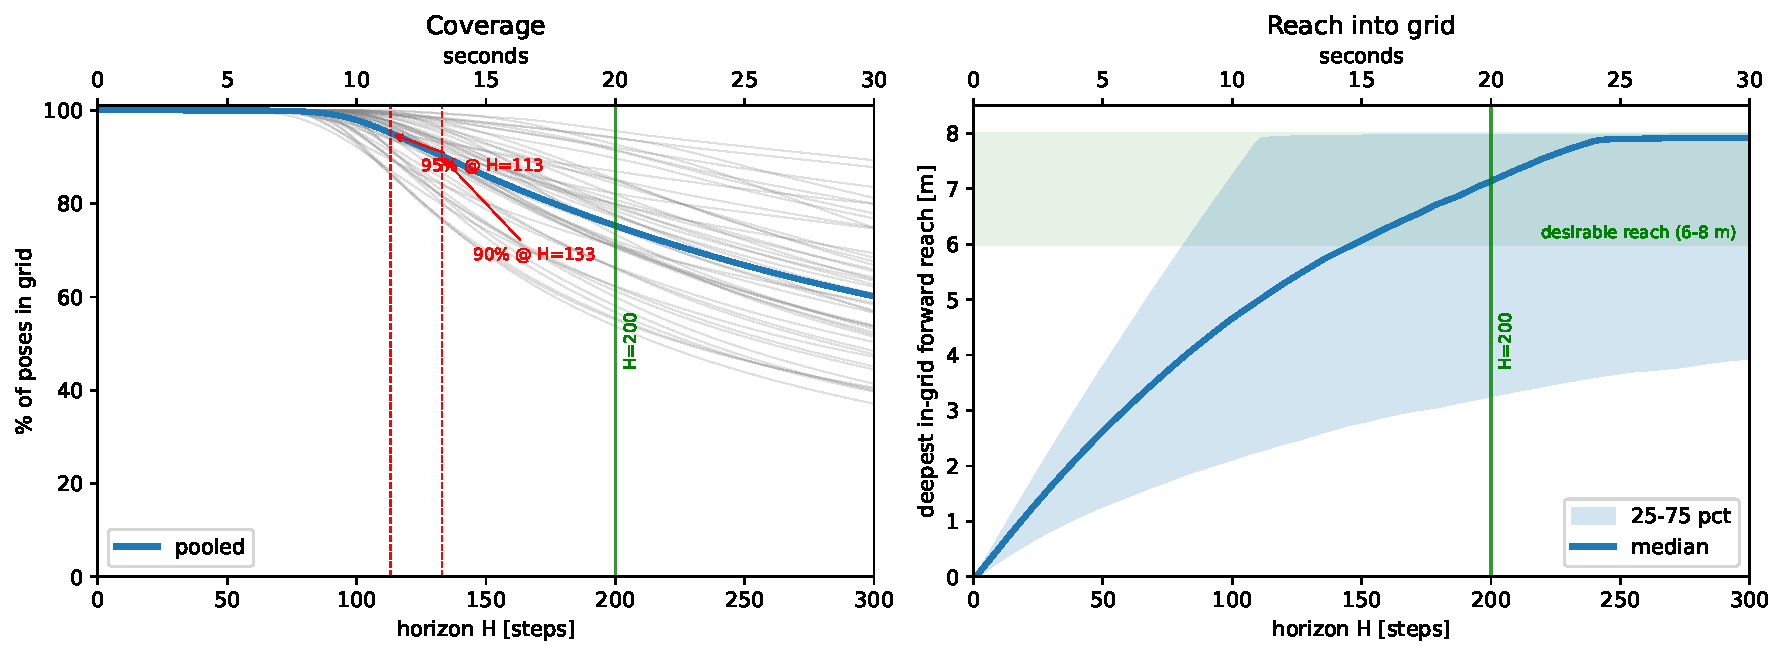
\includegraphics[width=\linewidth]{figures/horizon_tradeoff.pdf}
  \caption{Left: fraction of supervised poses that land inside the BEV grid as a
    function of horizon (blue = pooled over all missions, grey = individual
    missions). Right: deepest in-grid forward reach (median and inter-quartile
    band); the shaded band marks the desirable $6$ to $8\,$m far region. The
    green line marks the adopted horizon $H = 180$. Coverage falls as reach
    rises, which sets up the trade-off discussed in Section~\ref{sec:horizon}.}
  \label{fig:horizon}
\end{figure}

\begin{table}[htbp]
\caption{Prediction-horizon trade-off, pooled over all 48 missions. Coverage is the fraction of supervised poses inside the grid; reach is the deepest in-grid forward distance the path attains. The last two columns give the fraction of anchors whose path reaches the mid (4\,m) and far (6\,m) grid.}
\label{tab:horizon}
\begin{tabular}{rrrrrr}
\toprule
$H$ & seconds & coverage [\%] & median reach [m] & $\ge 4$\,m [\%] & $\ge 6$\,m [\%] \\
\midrule
50 & 5.0 & 100.0 & 2.62 & 17.8 & 0.0 \\
75 & 7.5 & 99.9 & 3.72 & 46.4 & 16.5 \\
100 & 10.0 & 97.9 & 4.66 & 56.7 & 37.4 \\
125 & 12.5 & 92.2 & 5.44 & 62.3 & 45.5 \\
150 & 15.0 & 86.0 & 6.07 & 65.8 & 50.5 \\
185 & 18.5 & 78.2 & 6.82 & 69.0 & 55.8 \\
200 & 20.0 & 75.3 & 7.14 & 70.1 & 57.4 \\
225 & 22.5 & 70.8 & 7.63 & 71.6 & 59.3 \\
250 & 25.0 & 66.8 & 7.90 & 72.9 & 60.8 \\
275 & 27.5 & 63.2 & 7.91 & 73.8 & 62.0 \\
300 & 30.0 & 60.1 & 7.92 & 74.6 & 63.1 \\
\bottomrule
\end{tabular}
\end{table}


